\documentclass[10pt]{beamer}
\usepackage[utf8]{inputenc}
\usepackage{listings}
\usepackage{xcolor}

\usepackage{amsmath}
\usepackage{nccmath}
%\usepackage{showframe}
\usepackage{amssymb} 
\usetheme[progressbar=frametitle]{metropolis}
\usepackage{appendixnumberbeamer}
\usepackage{booktabs}
\usepackage[scale=2]{ccicons}

\usepackage{pgfplots}
\usepgfplotslibrary{dateplot}

\usepackage{xspace}
\newcommand{\themename}{\textbf{\textsc{metropolis}}\xspace}

\title{6 Algorithmic Journeys with Concepts}
%\subtitle{Generic algorithms and performance}
% \date{\today}
\date{}
\author{Taras Shevchenko}
\institute{Rails Reactor / Giphy}
% \titlegraphic{\hfill\includegraphics[height=1.5cm]{logo.pdf}}
\lstdefinestyle{cpp}{
  language=C++,
  stepnumber=1,
  numbersep=10pt,
  tabsize=2,
  showspaces=false,
  showstringspaces=false,
  basicstyle=\scriptsize,
  breaklines
}

\begin{document}

\maketitle

%\begin{frame}{Table of contents}
%  \setbeamertemplate{section in toc}[sections numbered]
%  \tableofcontents[hideallsubsections]
%\end{frame}


\begin{frame}{The Software Industry is Not Industrialized}
    \begin{columns}
        \begin{column}{0.6\textwidth}
			Software components (routines), to be widely applicable to
			different machines and users, should be available in families arranged
			according to precision, robustness, generality and time-space performance.
        \end{column}
        \begin{column}{0.4\textwidth}  %%<--- here
                \begin{center}
					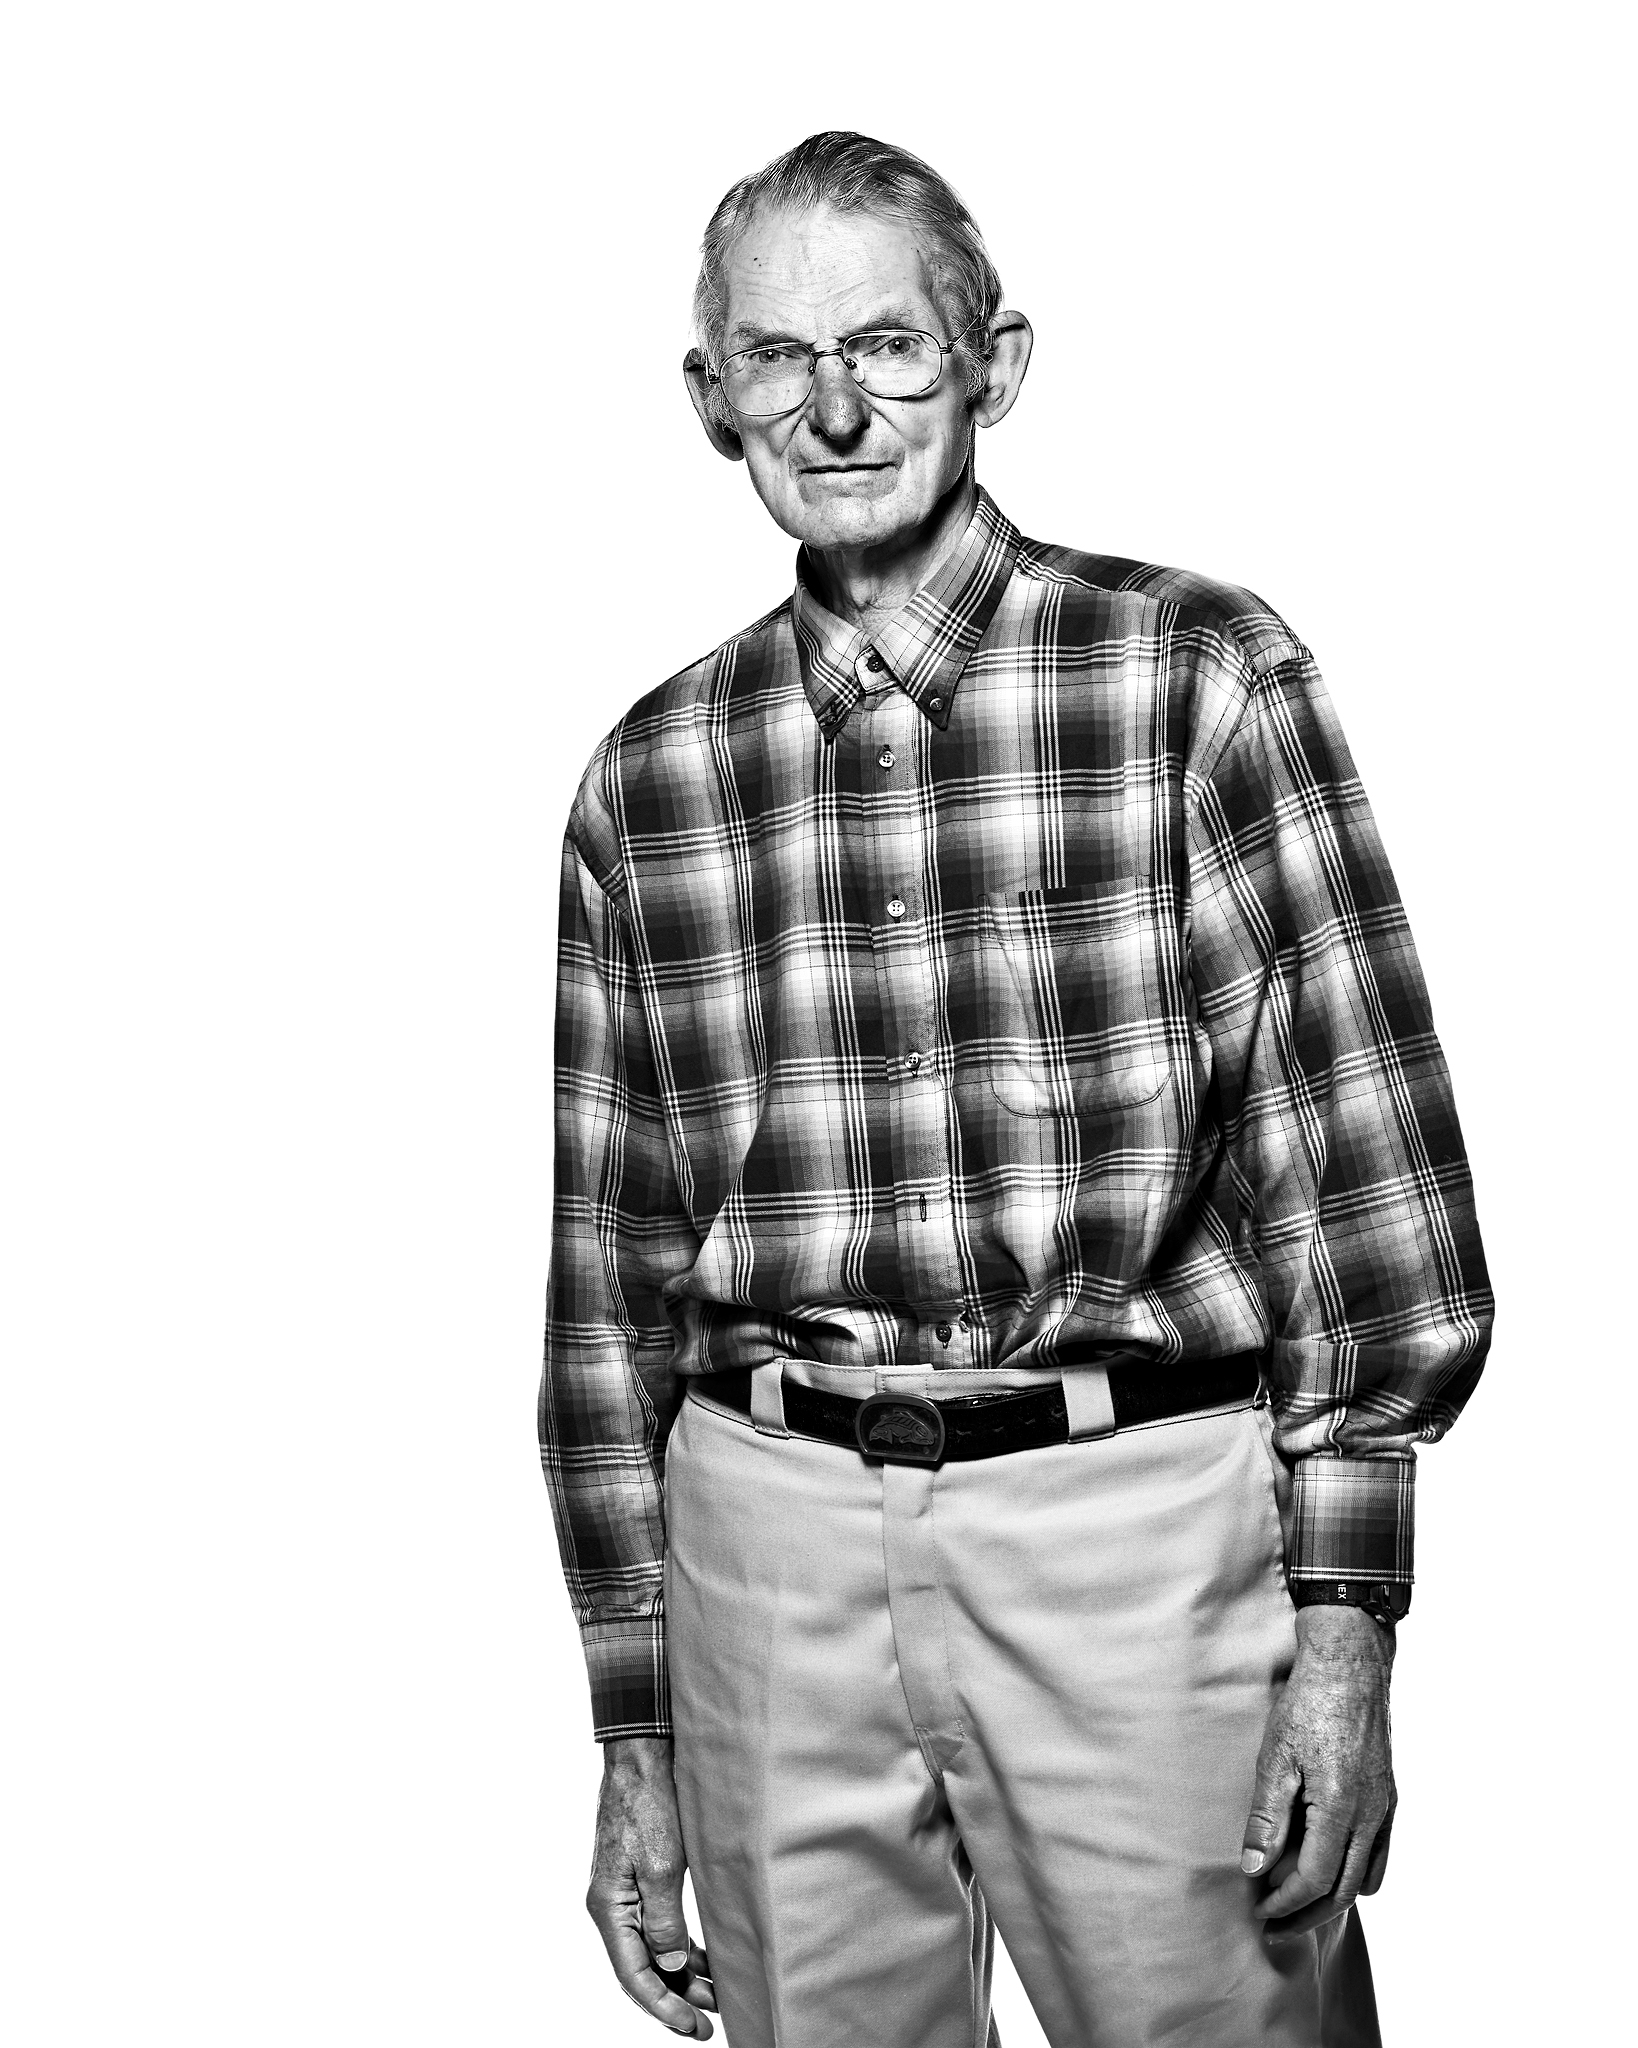
\includegraphics[height=5cm]{images/doug_mcilroy.jpg}
                \end{center}
        \end{column}
    \end{columns}
\end{frame}

\begin{frame}{A Familiar Example. Douglas McIlroy about sin}
Dimensions along which we wish to have variablity:
\begin{enumerate}
    \item precision, for which perhaps ten different approximating functionsmight suffice
    \item floating vs fixed computation
    \item argument ranges $[0, \pi/2]$, $[0, 2pi]$, also $[-\pi/2, pi/2]$, $[-\pi, \pi]$, $[-big, +big]$
    \item robustness - ranging from no argument validation through signaling of complete loss of significance, to signaling of specified range violations
\end{enumerate}

\end{frame}

\begin{frame}{Douglas McIlroy}
    \begin{columns}
        \begin{column}{0.6\textwidth}
            \begin{enumerate}
                \item Choices
                    \begin{enumerate}
                        \item precision
                        \item robustness
                        \item generality
                        \item generality
                        \item algorithm
                        \item interfaces and error-handling
                    \end{enumerate}
                \item Application Areas
                \begin{enumerate}
                    \item numerical approximation
                    \item I/O
                    \item 2d and 3d geometry
                    \item text processing
                    \item storage management
                \end{enumerate}
            \end{enumerate}

        \end{column}
        \begin{column}{0.4\textwidth}  %%<--- here
                \begin{center}
					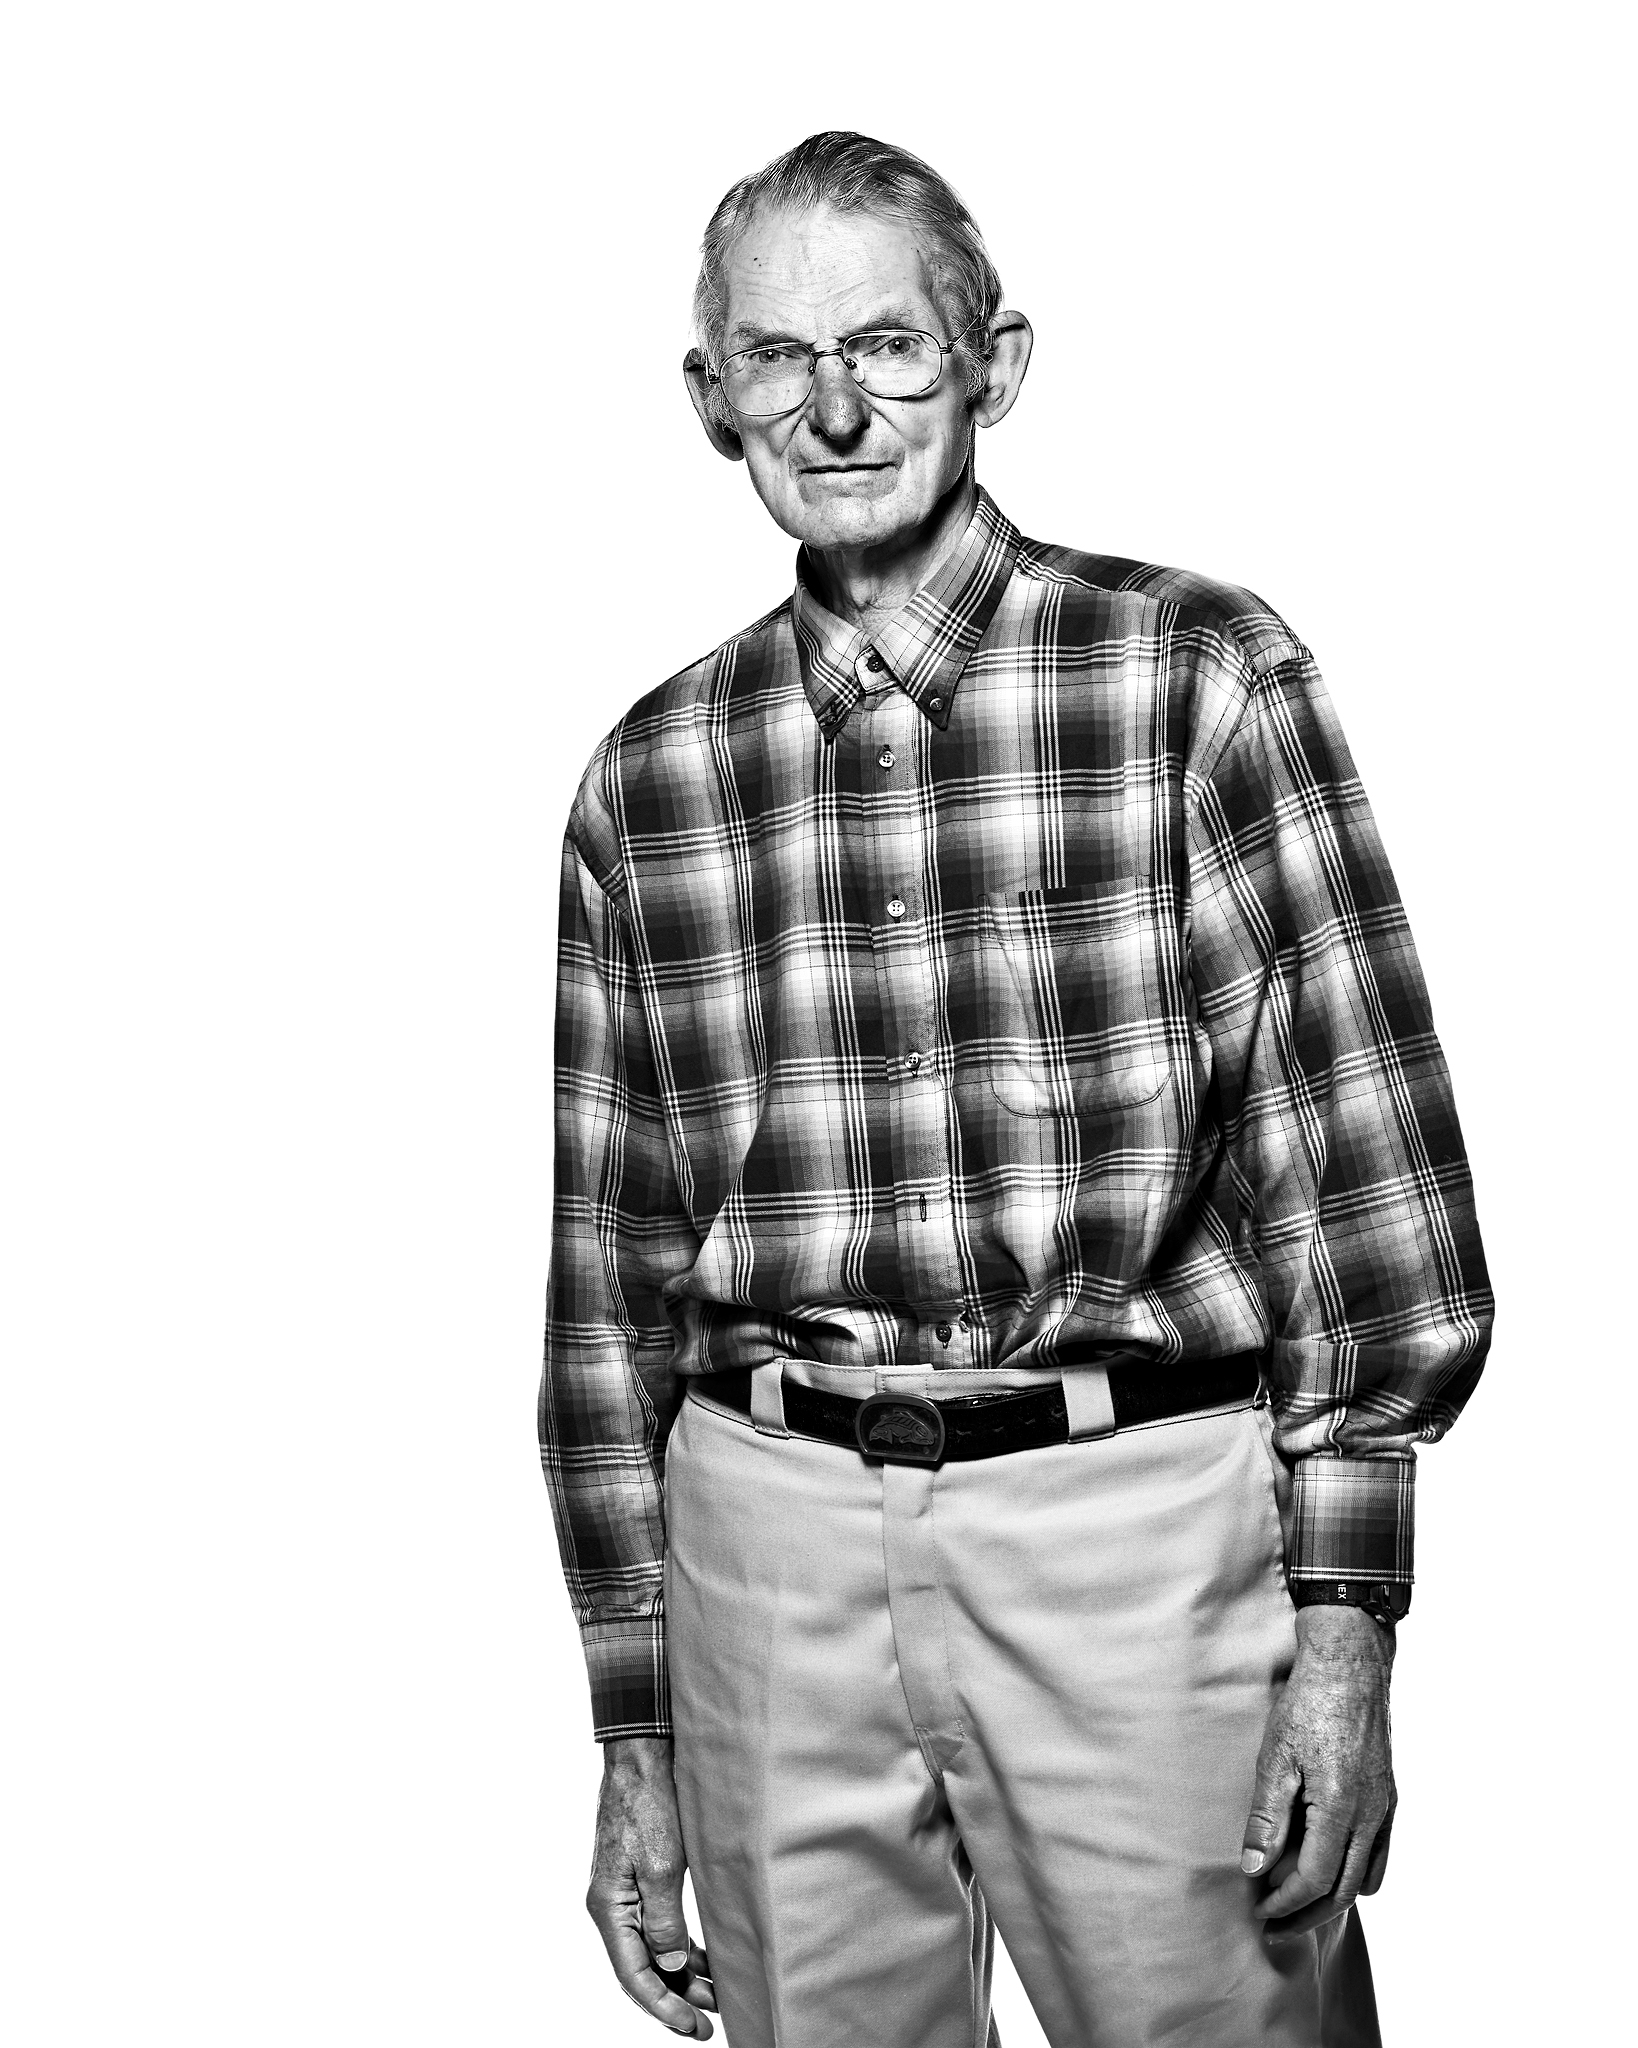
\includegraphics[height=5cm]{images/doug_mcilroy.jpg}
                \end{center}
        \end{column}
    \end{columns}
\end{frame}


\begin{frame}{Donald Knuth}
    \begin{columns}
        \begin{column}{0.6\textwidth}
            \begin{enumerate}
                \item Fundamental Algorithms
                \item Seminumerical Algorithms
                \item Sorting and Searching
                \item Combinatorial Algorithms
                \item Syntactic Algorithms
                \item The Theory of Context-free Languages
                \item Compiler Techniques
            \end{enumerate}
        \end{column}
        \begin{column}{0.4\textwidth}  %%<--- here
                \begin{center}
					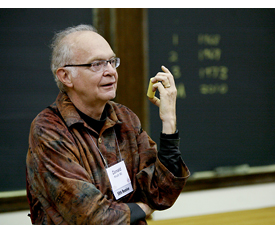
\includegraphics[height=3.5cm]{images/knuth.jpg}
                \end{center}
        \end{column}
    \end{columns}
\end{frame}

\begin{frame}{Niklaus Wirth}
    \begin{columns}
        \begin{column}{0.6\textwidth}
	        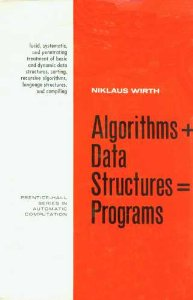
\includegraphics[height=7cm]{images/algorithms_data_structures_programs.jpg}
        \end{column}
        \begin{column}{0.4\textwidth}  %%<--- here
                \begin{center}
					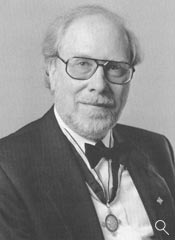
\includegraphics[height=5cm]{images/wirth.jpg}
                \end{center}
        \end{column}
    \end{columns}
\end{frame}


\begin{frame}{John Backus}
    \begin{columns}
        \begin{column}{0.6\textwidth}
            \begin{figure}
    	        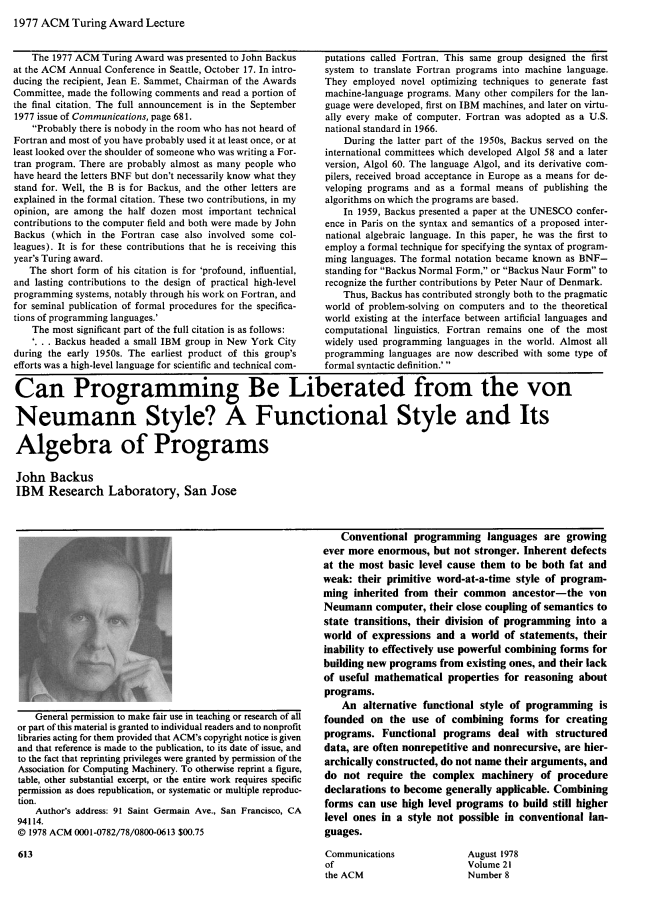
\includegraphics[height=6cm]{images/functional.png}
	    	    \caption{We need a few functional forms}
            \end{figure}
        \end{column}
        \begin{column}{0.4\textwidth}  %%<--- here
                \begin{center}
					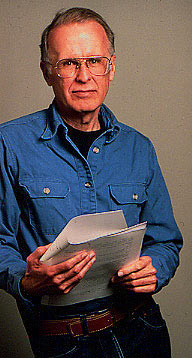
\includegraphics[height=5cm]{images/backus.jpg}
                \end{center}
        \end{column}
    \end{columns}
\end{frame}





\begin{frame}{Dmitri Mendeleev}
    \begin{columns}
        \begin{column}{0.6\textwidth}
			\begin{figure}
				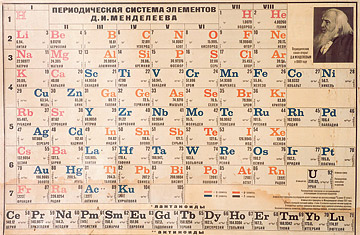
\includegraphics[height=4cm]{images/periodic_table.jpg}
				\caption{A Russian periodic table based on Dmitri Mendeleyev's original table of 1869.}
			\end{figure}
        \end{column}
        \begin{column}{0.4\textwidth}  %%<--- here
                \begin{center}
					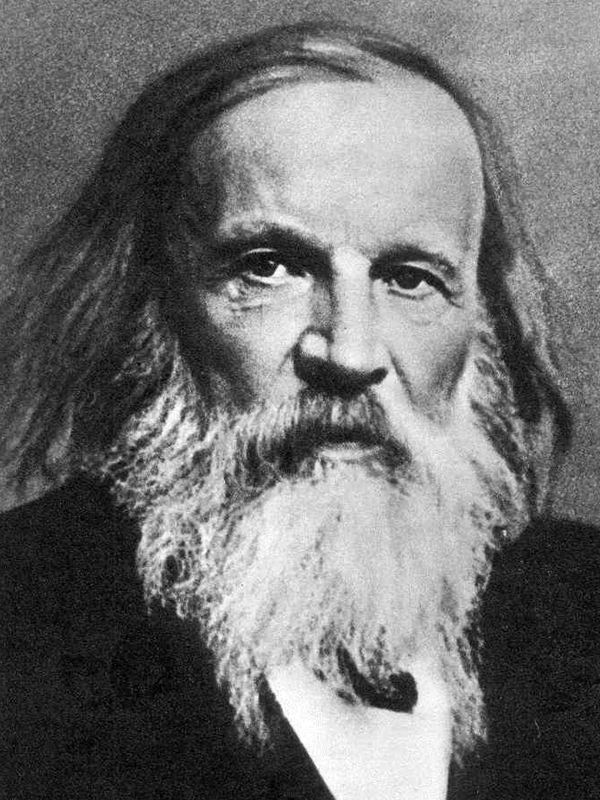
\includegraphics[height=5cm]{images/mendeleev.jpg}
                \end{center}
        \end{column}
    \end{columns}
\end{frame}



\begin{frame}{Carl Linnaeus}
    \begin{columns}
        \begin{column}{0.6\textwidth}
			Species Plantarum lists every species of plant known at the time, classified into genera. It is the first work to consistently apply binomial names and was the starting point for the naming of plants.
        \end{column}
        \begin{column}{0.4\textwidth}  %%<--- here
                \begin{center}
					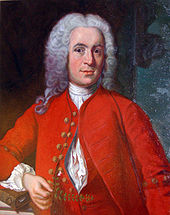
\includegraphics[height=5cm]{images/LinnaeusWeddingPortrait.jpg}
                \end{center}
        \end{column}
    \end{columns}
\end{frame}


\begin{frame}{Euclid}
	\begin{columns}
        \begin{column}{0.6\textwidth}
			\begin{enumerate}
				\item Definitions
				\item Postulates
				\item Common notions
			\end{enumerate}
		\end{column}
        \begin{column}{0.4\textwidth}  %%<--- here
                \begin{center}
					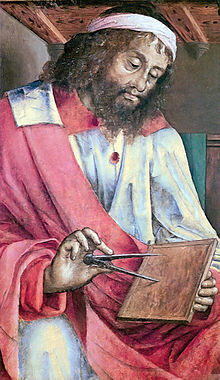
\includegraphics[height=5cm]{images/euclid.jpg}
                \end{center}
        \end{column}
	\end{columns}
\end{frame}

\begin{frame}{Common Notions}
\begin{enumerate}
	\item Things which are equal to the same thing are also equal to one other.
	\item If equals be added to equals, the wholes are equal.
	\item If equals be subructed from equals, the remainders are equal.
	\item Things which coincide with one another are equal to one another.
	\item The whole is greater than the part.
\end{enumerate}
\end{frame}



\begin{frame}{Basic idea}
\begin{block}{}
The essence of generic programming lies in the idea of concepts. A concept is a way of describing a family of related object types.
\end{block}
\begin{center}
    \begin{tabular}{ | p{1.5cm} | l | l | p{3cm} |}
    \hline
    \textbf{Natural Science} & \textbf{Mathematics} & \textbf{Programming} & \textbf{Programming Examples} \\ \hline
      genus & theory & concept & Integral, Character \\ \hline
      species & model & type or class & uint8\_t, char \\ \hline
      individual & element & instance  & 01000001(65, 'A') \\
    \hline
    \end{tabular}
\end{center}
\end{frame}


\begin{frame}[fragile]{Definitions}
  \begin{enumerate}
    \item Datum
    \item Value
    \item Value type
    \item Object
    \item Object type
  \end{enumerate}
\end{frame}



\begin{frame}[fragile]{Datum}
\begin{block}{Definition}
A \textbf{datum} is a sequence of bits.
\end{block}

\begin{block}{Example}
01000001 is an example of a datum.
\end{block}

\end{frame}

\begin{frame}[fragile]{Value}
\begin{block}{Definition}
A \textbf{value is} a \textbf{datum} together with its interpretation.
\end{block}
\begin{block}{Example}
The \textbf{datum} 01000001 might have the interpretation of the integer 65, or the character “A".
\end{block}
\begin{block}{Explanation}
Every \textbf{value} must be associated with a \textbf{datum} in memory; there is no way to refer to disembodied \textbf{values} in modern programming languages.
\end{block}
\end{frame}

\begin{frame}[fragile]{Value type}
\begin{block}{Definition}
A \textbf{value type} is a set of values sharing a common interpretation.
\end{block}
\end{frame}

\begin{frame}[fragile]{Object}
\begin{block}{Definition}
An \textbf{object} is a collection of bits in memory that contain a \textbf{value} of a given \textbf{value type}.
\end{block}
\begin{block}{Explanation}
An \textbf{object} is immutable if the value never changes, and mutable otherwise. An object is unrestricted if it can contain any \textbf{value} of its \textbf{value type}.
\end{block}
\end{frame}


\begin{frame}[fragile]{Object type}
\begin{block}{Definition}
An \textbf{object type} is a uniform method of storing and retrieving \textbf{values} of a given \textbf{value type} from a particular \textbf{object} when given its address.
\end{block}
\end{frame}

\section{Programming with concepts}
\begin{frame}{Semiregular}
    \begin{block}{Operation}
      \begin{enumerate}
        \item Copy construction
        \item Assignment
        \item Destruction
      \end{enumerate}
    \end{block}

    \begin{block}{Semantic}
        $$\forall a ~ \forall b ~ \forall c : T~a(b)  \implies(b = c \implies a = c)$$
        $$\forall a ~ \forall b ~ \forall c : a \leftarrow b  \implies(b = c \implies a = c)$$
        $$\forall f \in RegularFunction: a = b \implies f(a) = f(b)$$
    \end{block}
\end{frame}

\begin{frame}[fragile]{Semiregular}
\begin{lstlisting}[style=cpp]

template<typename T>
concept semiregular = std::is_default_constructible<T>::value &&
                      std::is_copy_constructible<T>::value &&
                      std::is_copy_assignable<T>::value &&
                      std::is_destructible<T>::value

\end{lstlisting}
\end{frame}

\begin{frame}{Regular type}
\begin{block}{Operation}
  \begin{enumerate}
    \item Copy construction
    \item Assignment
    \item Equality
    \item Destruction
  \end{enumerate}
\end{block}
\begin{block}{Semantic}
    $$\forall a ~ \forall b ~ \forall c : T~a(b)  \implies(b = c \implies a = c)$$
    $$\forall a ~ \forall b ~ \forall c : a \leftarrow b  \implies(b = c \implies a = c)$$
    $$\forall f \in RegularFunction: a = b \implies f(a) = f(b)$$
\end{block}
\end{frame}

\begin{frame}[fragile]{Regular}
\begin{lstlisting}[style=cpp]

template<typename T>
concept semiregular = semiregular<T> && is_equality_comparable<T>::value;

\end{lstlisting}
\end{frame}

\begin{frame}{Relation}
    \begin{align*}
        FunctionalProcedure(F) \triangleq F~is~a~regular~procedure~defined~on~regular~&\\
        types:~replacing~its~inputs~with~equal~objects~\\
        results~in~equal~output~objects. \\\\
        HomogeneousFunction(F) \triangleq FunctionalProcedure(F) \land Arity(F) > 0\\
        \land (\forall i,j \in \mathbb{N})(i,j < Arity(F)) \implies (InputType(F, i) = InputType(F, j))\\
        \land Domain: HomogeneousFunction \rightarrow Regular\\
        F \implies InputType(F, 0)
    \end{align*}
\end{frame}



\begin{frame}[fragile]{Regular}
\begin{lstlisting}[style=cpp]
template<typename F, typename... T>
concept functional_procedure = (regular<typename std::invoke_result<F, T...>::type> || std::is_same<typename std::invoke_result<F, T...>::type, void>::value) && is_regular<T...>::value;

template<typename F, typename... T>
concept homogeneous_function = functional_procedure<F, T...> && sizeof...(T) > 0 && all_same<T...>::value && all_regular<T>;

\end{lstlisting}
\end{frame}



\begin{frame}
\begin{align*}
    Predicate(P) \triangleq FunctionalProcedure(F) \land Codomain(P) = bool\\\\
    HomogeneousPredicate(P) \triangleq Predicate(P) \land HomogeneousFunction(P) \\\\
    Relation(R) \triangleq HomogeneousPredicate(R) \land Arity(R) = 2\\\\
\end{align*}

\end{frame}


\begin{frame}[fragile]{Relation}
\begin{lstlisting}[style=cpp]
template<typename F, typename... T>
concept predicate = functional_procedure<F, T...> && std::is_same<codomain_t<F, T...>, bool>::value;

template<typename F, typename... T>
concept homogeneous_predicate = predicate<F, T...> && homogeneous_function<T...>;

template<typename R, typename T>
concept relation = predicate<R, T, T>;
\end{lstlisting}
\end{frame}


\begin{frame}{Totally Ordered}
    \begin{align*}
        property(R: Relation)\\
        transitive: R \\
                r \mapsto (\forall a,b,c \in Domain(R)) (r(a, b) \land r(b,c) \implies r(a, c))\\\\
        property(R: Relation)\\
        total\_ordering: R \\
                r \mapsto transitive(r)~\land(\forall a,b \in Domain(R))~exactly~one~of~following~holds:\\
            r(a, b),~r(b, a),~or~a = b\\
    \end{align*}

    \begin{align*}
        TotallyOrdered(T) \triangleq Regular(T) \land <: T~x~T \rightarrow bool \land total\_ordering(<)
    \end{align*}
\end{frame}

\begin{frame}[fragile]{Totally Ordered}
\begin{lstlisting}[style=cpp]
template<typename T>
concept totally_ordered = regular<T> && is_less_than_comprable<T>::value;

\end{lstlisting}
\end{frame}



\begin{frame}{Concepts}
    \begin{align*}
        Readable(T) ~\triangleq~ & Regular(T) ~\land \\
        & ValueType: Readable \rightarrow Regular ~\land \\
        & source: T \rightarrow ValueType(T) ~\land\\
    \end{align*}
\end{frame}

\begin{frame}{Concepts}
    \begin{align*}
        Writable(T) ~\triangleq~ & Regular(T) ~\land \\
        & ValueType: Writable \rightarrow Regular ~\land \\
        & (\forall x \in T) (\forall v \in ValueType(T))~sink(x)~\leftarrow~v ~ \\
        & ~~~~is~a~well-formed~statement \\
        & source: T \rightarrow ValueType(T) ~\land\\
    \end{align*}
\end{frame}


\begin{frame}{Concepts}
    \begin{align*}
        Iterator(T) ~\triangleq~ & Regular(T) ~\land \\
        & DistanceType: Iterator \rightarrow Integer ~\land \\
        & successor: T \rightarrow T ~\land\\
        & successor~is~not~necessarily-regular
    \end{align*}
\end{frame}

\begin{frame}{Concepts}
    \begin{align*}
        ForwardIterator(T) ~\triangleq~ & Iterator(T) ~\land ~regular\_unary\_function(successor)
    \end{align*}
\end{frame}

\begin{frame}{Concepts}
    \begin{align*}
        BidirectionalIterator(T) ~\triangleq~ & ForwardIterator(T) ~\land \\
                                              & predecessor: T \rightarrow T ~\land \\
                                              & predecessor~takes~constant~type ~\land \\
                                              & (\forall i \in T) successor(i) is defined~\implies \\
                                              & ~~~~predecessor(successor(i))~is~defined \\
                                              & ~~~~and~equals~to~i~ \land\\
                                              & (\forall i \in T) predecessor(i)~is~defined~ \implies \\
                                              & ~~~~successor(predecessor(i))~is~defined\\
                                              & ~~~~and~equals~to~i
    \end{align*}
\end{frame}

\begin{frame}{Concepts}
    \begin{align*}
        IndexedIterator(T) ~\triangleq~ & ForwardIterator(T) ~\land \\
                                              & +: T~x~DifferenceType(T) \rightarrow T ~\land\\
                                              & -: T~x~T \rightarrow DifferenceType(T) ~\land\\
                                              & + takes~constant~time\\
                                              & - takes~constant~time
    \end{align*}
\end{frame}


\begin{frame}{Concepts}
    \begin{align*}
        RandomAccessIterator(T)  ~\triangleq~ & BidirectionalIterator(T) ~\land \\
                                              & IndexedIterator(T) ~\land \\
                                              & TotallyOrdered(T) ~\land \\
                                              & (\forall i,j \in T) ~i < j \iff i \prec j ~ \land \\
                                              & DifferenceType: \\
                                              & ~~~~RandomAccessIterator \rightarrow Integer ~ \land\\
                                              & +: T~x~DifferenceType(T) \rightarrow T ~\land\\
                                              & -: T~x~DifferenceType(T) \rightarrow T ~\land\\
                                              & -: T~x~T \rightarrow DifferenceType(T) ~\land\\
                                              & < takes~constant~time ~\land\\
                                              & - between~and~iterator~and~an~integer \\
                                              & ~~~~takes~constant~time
    \end{align*}
\end{frame}

\begin{frame}{Concepts}
    \begin{align*}
        FunctionalProcedure(F) \triangleq F~is~a~regular~procedure~defined~on~regular~&\\
        types:~replacing~its~inputs~with~equal~objects~\\
        results~in~equal~output~objects.
    \end{align*}
    \begin{align*}
        UnaryFunction(F) \triangleq FunctionalProcedure(F) \land Arity(F) = 1 &\\
                \land~Domain: UnaryFunction \rightarrow Regular &\\
                F \mapsto InputType(F, 0)
    \end{align*}
    \begin{align*}
        HomogeneousFunction(F) \triangleq FunctionalProcedure(F) \land Arity(F) > 0\\
        \land (\forall i,j \in \mathbb{N})(i,j < Arity(F)) \implies (InputType(F, i) = InputType(F, j))\\
        \land Domain: HomogeneousFunction \rightarrow Regular\\
        F \implies InputType(F, 0)
    \end{align*}
\end{frame}

\begin{frame}{Concepts}
    \begin{align*}
        Predicate(P) \triangleq FunctionalProcedure(F) \land Codomain(P) = bool
    \end{align*}
    \begin{align*}
        HomogeneousPredicate(P) \triangleq Predicate(P) \land HomogeneousFunction(P)
    \end{align*}
    \begin{align*}
        Relation(R) \triangleq HomogeneousPredicate(R) \land Arity(R) = 2
    \end{align*}
\end{frame}
\begin{frame}{}
    \begin{align*}
        property(R: Relation)\\
        total\_ordering: R \\
                r \mapsto transitive(r)~\land(\forall a,b \in Domain(R))~exactly~one~of~following~holds:\\
            r(a, b),~r(b, a),~or~a = b\\
    \end{align*}
\end{frame}

\begin{frame}{Journey 1}
    \begin{enumerate}
        \item min
        \item max
    \end{enumerate}
\end{frame}

\begin{frame}{Journey \#1}
    \begin{block}{}
		\lstinputlisting[language=c++]{code/snippets/1/0.min.0.h}
	\end{block}
\end{frame}

\begin{frame}{Journey \#1}
    \begin{block}{}
		\lstinputlisting[language=c++]{code/snippets/1/0.min.1.h}
	\end{block}
\end{frame}


\begin{frame}{Journey \#1}
    \begin{block}{}
		\lstinputlisting[language=c++]{code/snippets/1/0.min.2.h}
	\end{block}
\end{frame}

\begin{frame}{Journey \#1}
    \begin{block}{Dealing with large objects}
		\lstinputlisting[language=c++]{code/snippets/1/0.min.3.h}
	\end{block}
\end{frame}

\begin{frame}{Journey \#1}
    \begin{block}{}
		\lstinputlisting[language=c++]{code/snippets/1/0.min.4.h}
	\end{block}
\end{frame}

\begin{frame}{Journey \#1}
    \begin{block}{}
		\lstinputlisting[language=c++]{code/snippets/1/0.min.5.cpp}
	\end{block}
\end{frame}

\begin{frame}{Journey \#1}
    \begin{block}{}
		\lstinputlisting[language=c++]{code/snippets/1/0.min.6.h}
	\end{block}
\end{frame}

\begin{frame}{Journey \#1}
    \begin{block}{}
		\lstinputlisting[language=c++]{code/snippets/1/0.min.7.h}
	\end{block}
\end{frame}
\begin{frame}{Journey \#1}
    \begin{block}{}
		\lstinputlisting[language=c++]{code/snippets/1/0.min.8.h}
	\end{block}
\end{frame}

\begin{frame}{Journey \#1}
    \begin{block}{}
		\lstinputlisting[language=c++]{code/snippets/1/0.max.0.h}
	\end{block}
\end{frame}

\begin{frame}{Journey \#1}
    \begin{block}{}
		\lstinputlisting[language=c++]{code/include/cppcon/cppcon.function.min0.h}
	\end{block}
\end{frame}

\begin{frame}{Journey \#2}
    \begin{enumerate}
        \item unique
        \item unique\_count
    \end{enumerate}
\end{frame}

\begin{frame}{Journey \#2}
    \begin{block}{}
		\lstinputlisting[language=c++,firstline=2]{code/include/cppcon/cppcon.function.unique.0.h}
	\end{block}
\end{frame}



\begin{frame}{Journey \#3}
    \begin{enumerate}
        \item frequencies 
        \item transform\_subgroups
        \item squash\_subgroups
    \end{enumerate}
\end{frame}

\begin{frame}{Journey \#4}
    \begin{enumerate}
        \item split
        \item transform\_splits
    \end{enumerate}
\end{frame}

\begin{frame}{Journey \#5}
    \begin{enumerate}
        \item remove\_if
        \item partition\_semistable
    \end{enumerate}
\end{frame}


\begin{frame}{More examples of concepts}
\begin{enumerate}
  \item Regular Type
  \item Semiegular Type
  \item Functional Procedure
  \item Homogeneous Function
  \item Homogeneous Predicate
  \item Semiring
  \item Sequence
  \item Totally Ordered
  \item Input Iterator
  \item Forfward Iterator
  \item Bidirectional Iterator
\end{enumerate}
\end{frame}

\begin{frame}{Properties}
\begin{enumerate}
  \item Associative
  \item Distributive
  \item Transitive
  \item Semiegular Type
  \item Functional Procedure
\end{enumerate}
\end{frame}

\begin{frame}{Techniques}
\begin{enumerate}
  \item Transformation-action duality
  \item Operation-accumulation procedure duality
  \item Memory adaptivity
  \item Reduction to constrained subproblem 
\end{enumerate}
\end{frame}

\section{Conclusion}

\begin{frame}{Conclusion}
  \begin{enumerate}
    \item Concepts are mathematical. They are not specific to C++.
    \item Know as many algorithms as you can.
    \item Algorithms come in groups.
    \item Transform complicated loops into well-defined algorithms.
    \item Use mathematics for everything you do.
    \item Don't obay mathematical convetions in programming.
    \item Prefare concrete algorithms to more general.
    \item Have a little Euclid, Knuth, Dijkstra in your mind and let them argue.
  \end{enumerate}
\end{frame}

\end{document}
